\begin{exercise}{2016/17 4}
    \emph{Το απλό εκκρεμές} είναι το σύστημα, σε κανονική μορφή,
    \begin{align*}
        \dot{x} &= y \\
        \dot{y} &= -a y - \sin{x}
    \end{align*}
    και περιγράφει ένα απλό εκκρεμές, αλλά και τη δυναμική ενός περιστρεφόμενου
    σώματος γύρω από έναν άξονα.

    Για μηδενική απόσβεση \( a = 0 \) το σύστημα είναι Χαμιλτονιανό. Για θετική
    απόσβεση \( a > 0 \), τα σημεία ισορροπίας δεν μετακινούνται, αλλά αλλάζει η
    ευστάθειά τους.

    \begin{enumerate}[label= (\alph*)]
        \item Δώστε τυπικά πορτρέτα κίνησης για διάφορες θετικές τιμές του
            \( a \) και περιγράψτε τις ποιοτικές αλλαγές στη δυναμική
            συμπεριφορά που παρατηρούνται.
        \item Εφαρμόζεται τώρα μία σταθερή ροπή \( T \) στο σύστημα, ώστε το
            σύστημα είναι
            \begin{align*}
                \dot{x} &= y \\
                \dot{y} &= -a y - \sin{x} + T.
            \end{align*}
            Τα σημεία ισορροπίας μετακινούνται.
            \begin{enumerate}[label= (\roman*)]
                \item Θεωρούμαι πρώτα την περίπτωση \( 0 < T < 1 \). Με κατάλληλη
                    αναφορά στο αντίστοιχο Χαμιλτονιανό σύστημα (δηλαδή για
                    \( a = 0 \), για το οποίο και κάνετε το πορτρέτο
                    κίνησης), δείξτε πως η περιοχή έλξης παραμένει μεν σταθερή, αλλά
                    είμαστε πολύ κοντά σε αστάθεια, καθώς το ευσταθές σημείο
                    πλησιάζει το σάγμα και χρειάζεται μικρή ενέργεια για να βγούμε
                    (και τι γίνεται μετά;).
                \item Δείξτε ότι για \( T > 1 \) δεν υπάρχουν σημεία ισορροπίας.
                    Το σύστημα παρ᾽ όλα αυτά παραμένει ευσταθές λόγω των
                    αποσβέσεων. Δώστε το πορτρέτο κίνησης και δείξτε ότι υπάρχει
                    ευσταθής οριακός κύκλος στον κύλινδρο (αυστηρή απόδειξη
                    γίνεται με χρήση του θεωρήματος των \tl{Poincar\'{e}-Bendixson}).
            \end{enumerate}
    \end{enumerate}
\end{exercise}
\begin{solution}{2016/17 4}
    (α). Τα σημεία ισορροπίας του απλού εκκρεμούς υπολογίζονται από
    \begin{align*}
        0 &= y \\
        0 &= -a y - \sin{x},
    \end{align*}
    που σημαίνει ότι \( x = k\pi \) με \( k \in \mathbb{Z} \). Αν γράψουμε τις
    σχέσεις στη μορφή
    \[
        \begin{pmatrix}
            \dot{x} \\
            \dot{y}
        \end{pmatrix} = F(x, y) =
        \begin{pmatrix}
            y \\
            -a y - \sin{x}
        \end{pmatrix},
    \]
    και πάρουμε τη γραμμικοποίηση προκύπτει
    \[
        DF(x, y) =
        \begin{pmatrix}
            0 & 1 \\
            -\cos{x} & -a
        \end{pmatrix}.
    \]
    Στο \( (0, 0) \) ή γενικότερα στο \( (2k\pi, 0) \) ισχύει
    \[
        DF(2k\pi, 0) =
        \begin{pmatrix}
            0 & 1 \\
            -1 & -a
        \end{pmatrix},
    \]
    και οι ιδιοτιμές της είναι
    \[
        \det
        \begin{pmatrix}
            -\lambda & 1 \\
            -1 & -a - \lambda
        \end{pmatrix}
        = \lambda^2 + \lambda a + 1.
    \]
    Η παραπάνω έχει διακρίνουσα
    \[
        \Delta = a^2 - 4.
    \]
    Όταν \( \Delta < 0 \), δηλαδή όταν \( 0 < a < \sqrt{2} \) τότε οι ρίζες
    \[
        \lambda = \frac{-a \pm i \sqrt{a^2 - 4}}{2},
    \]
    είναι μιγαδικές με αρνητικό πραγματικό μέρος και συνεπώς από το θεώρημα
    \tl{Hartman-Grobman} το σημείο είναι ασυμπτωτικά ευσταθές για το μη-γραμμικό
    σύστημα, για \( a > 0 \) και έχει τη μορφή ευσταθούς εστίας. Όταν \( a = 0 \)
    δε μπορούμε να εφαρμόσουμε το θεώρημα, αλλά γνωρίζουμε ότι έχει συμπεριφορά
    κέντρου από τη μελέτη του Χαμιλτονιανού συστήματος καθώς στο \( 2k\pi \) η
    συνάρτηση δυναμικού παρουσιάζει ελάχιστο.

    Αν \( \Delta > 0 \) τότε εύκολα φαίνεται ότι
    \[
        \lambda_1 = \frac{-a + \sqrt{a^2 - 4}}{2} < 0, \quad
        \lambda_2 = \frac{-a - \sqrt{a^2 - 4}}{2} < 0.
    \]
    Συνεπώς από το θεώρημα \tl{Hartman-Grobman} το σημείο είναι
    ασυμπτωτικά ευσταθές για το μη-γραμμικό σύστημα, με μορφή ευσταθούς κόμβου.
    Αυτή η περίπτωση φυσικά εμφανίζεται μόνο όταν \( a > 0 \).

    Τέλος, για \( \Delta = 0 \) τότε \( a = \sqrt{2} \) και προκύπτει η διπλή
    ιδιοτιμή \( \lambda_{1,2} = \frac{-a}{2} \), που είναι φυσικά ασυμπτωτικά
    ευσταθής.

    Αντίστοιχα για τα σημεία ισορροπίας \( ((2k + 1)\pi, 0) \) από την γραμμικοποίηση προκύπτει
    \[
        DF((2k + 1)\pi, 0) = \begin{pmatrix}
            0 & 1 \\
            -1 & -a
        \end{pmatrix},
    \]
    και οι ιδιοτιμές της είναι
    \[
        \det
        \begin{pmatrix}
            -\lambda & 1 \\
            1 & -a - \lambda
        \end{pmatrix}
        = \lambda^2 + \lambda a - 1.
    \]
    Η παραπάνω έχει διακρίνουσα
    \[
        \Delta = a^2 + 4 > 0,
    \]
    και οι ιδιοτιμές είναι
    \[
        \lambda_1 = \frac{-a + \sqrt{a^2 + 4}}{2} > 0, \quad
        \lambda_2 = \frac{-a - \sqrt{a^2 + 4}}{2} < 0.
    \]
    Συνεπώς από το θεώρημα \tl{Hartman-Grobman} το σημείο είναι
    σάγμα για το μη-γραμμικό σύστημα.

    Στο σχήμα~\ref{fig:ex4_undampedPendComb} απεικονίζεται το πορτρέτο κίνησης
    του απλού εκκρεμούς, χωρίς απόσβεση και χωρίς κάποια εξωτερική ροπή.
    \begin{figure}[h]
        \centering
        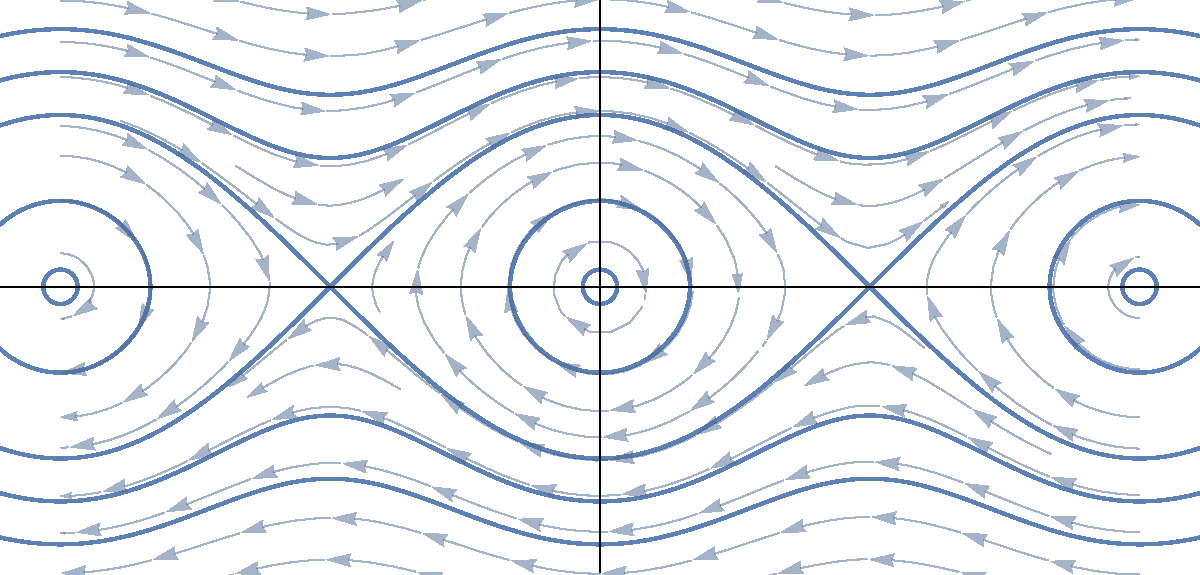
\includegraphics[width=0.8\textwidth]{figures/ex4_undampedPendComb.pdf}
        \caption{\gr{Πορτρέτο κίνησης εκκρεμούς, \( a = 0, T = 0 \)}}
        \label{fig:ex4_undampedPendComb}
    \end{figure}
    Το σύστημα στην περίπτωση αυτό είναι Χαμιλτονιανό με συνολική ενέργεια
    \[
        H(x, y) = \frac{1}{2}y^2 + U(x),\quad U(x) = - \cos{x}.
    \]
    Κοιτώντας το διάστημα \( (-\pi, \pi) \), βλέπουμε ότι στο \( (0, 0) \) έχουμε
    συμπεριφορά κέντρου και σημεία κοντά σε αυτό έχουν αυτή τη συμπεριφορά. Σημεία
    που βρίσκονται πάνω στις τροχιές των σαγμάτων ή πάνω από αυτές θα παραμείνουν
    για πάντα ασταθή και ποτέ δεν θα ισορροπήσουν. Επομένως, αυτό το
    \enquote*{μάτι} είναι η διαχωριστική καμπύλη (\tl{separatrix}). Τέλος, η
    τροχιά που τείνει στο \( \pi \) ή στο \( -\pi \) προέρχεται από την ευσταθή
    ιδιοτιμή και ουσιαστικά αντιπροσωπεύει την κάθετη θέση που δύναται να
    ισορροπήσει το εκκρεμές.

    Στο σχήμα~\ref{fig:ex4_damped05Comb}, απεικονίζεται το πορτρέτο κίνησης
    του απλού εκκρεμούς, με απόσβεση \( a = 0.5 \) και χωρίς κάποια εξωτερική ροπή.
    \begin{figure}[h]
        \centering
        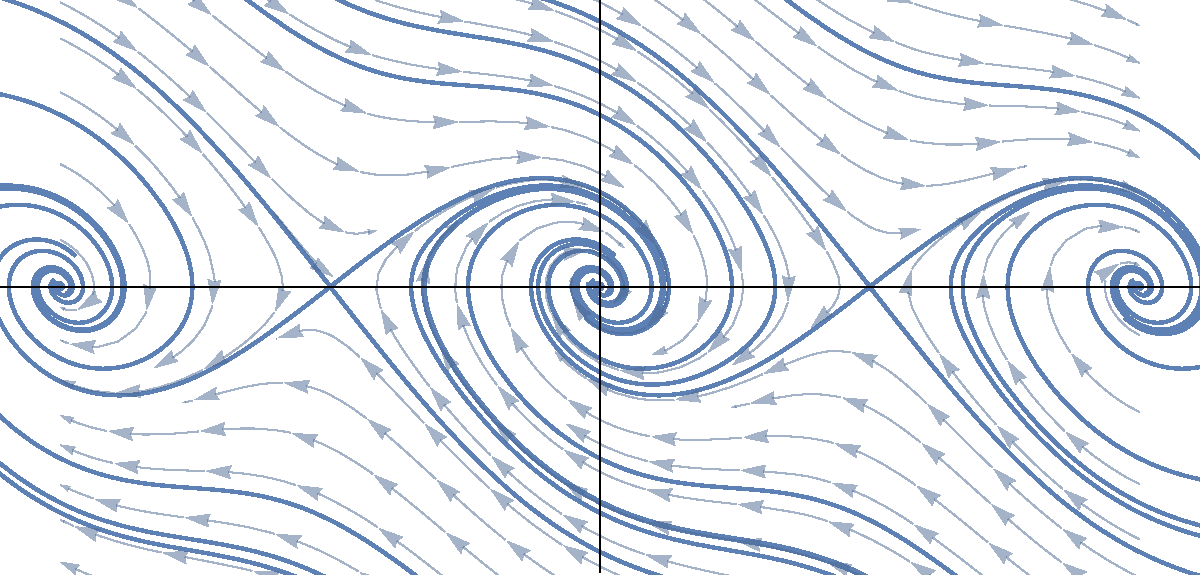
\includegraphics[width=0.8\textwidth]{figures/ex4_damped05Comb.pdf}
        \caption{\gr{Πορτρέτο κίνησης εκκρεμούς, \( a = 0.5, T = 0 \)}}
        \label{fig:ex4_damped05Comb}
    \end{figure}
    Όπως δείξαμε παραπάνω, και επικεντρώνοντας την προσοχή μας στο διάστημα
    \( (-\pi,\pi) \), η προσθήκη απόσβεσης μετατρέπει το σημείο \( (0, 0) \) από
    κέντρο σε ασυμπτωτικά ευσταθές σημείο ισορροπίας. Μία επιπλέον σημαντική αλλαγή
    που επιφέρει η απόσβεση είναι ότι αλλάζει (μεγαλώνει) την περιοχή έλξης. Όπως
    φαίνεται στο σχήμα~\ref{fig:ex4_damped05Comb}, οι τροχιές που τείνουν στο
    \( -\pi \) και \( \pi \) αντίστοιχα, είναι οι διαχωριστικές καμπύλες και
    είναι επίσης οι καμπύλες που αντιστοιχούν στην κάθετη θέση του εκκρεμούς.
    Η περιοχή έλξης για το σημείο ισορροπίας \( (0, 0) \) είναι αριστερά και
    δεξιά των διαχωριστικών καμπυλών του \( -\pi \) και \( \pi \) αντίστοιχα.

    Στο σχήμα~\ref{fig:ex4_damped1Comb}, απεικονίζεται το πορτρέτο κίνησης
    του απλού εκκρεμούς, με απόσβεση \( a = 1 \) και χωρίς κάποια εξωτερική ροπή.
    \begin{figure}[h]
        \centering
        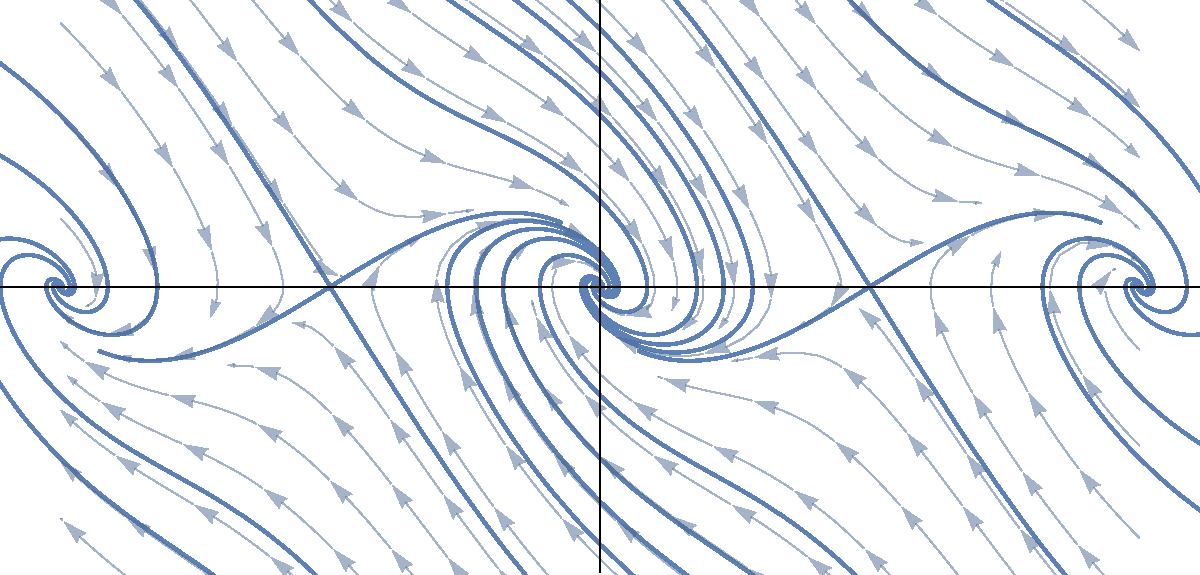
\includegraphics[width=0.8\textwidth]{figures/ex4_damped1Comb.pdf}
        \caption{\gr{Πορτρέτο κίνησης εκκρεμούς, \( a = 1, T = 0 \)}}
        \label{fig:ex4_damped1Comb}
    \end{figure}
    Δεν έχουμε κάποια ποιοτική αλλαγή σε σχέση με την περίπτωση όπου είχαμε
    \( a = 0.5 \). Δηλαδή ισχύει ότι και πριν. Η ουσιαστική διαφορά τους είναι
    ο ρυθμός σύγκλισης στο σημείο ισορροπίας. Με την αύξηση της απόσβεσης οι
    ταλαντώσεις μειώνονται αισθητά και αυτό αντικατοπτρίζεται στο
    σχήμα~\ref{fig:ex4_damped1Comb}.

    (β) \tl{i}. Περνάμε στην περίπτωση όπου εφαρμόζεται μία σταθερή ροπή
    \( T \) στο σύστημα, ώστε οι εξισώσεις να είναι
    \begin{align*}
        \dot{x} &= y \\
        \dot{y} &= -a y - \sin{x} + T,
    \end{align*}
    με \( 0 < T < 1 \). Υπολογίζοντας τα σημεία ισορροπίας προκύπτει
    \begin{align*}
        0 &= y \\
        0 &= -a y - \sin{x} + T,
    \end{align*}
    που συνεπάγεται
    \[
        \sin{x} = T.
    \]
    Η παραπάνω έχει τις λύσεις συναρτήσει τις ροπής
    \begin{align*}
        x_1(T) &= 2k\pi + \arcsin{T} \\
        x_2(T) &= (2k + 1)\pi - \arcsin{T},
    \end{align*}
    για \( k \in \mathbb{Z} \).
    \begin{figure}[h]
        \centering
        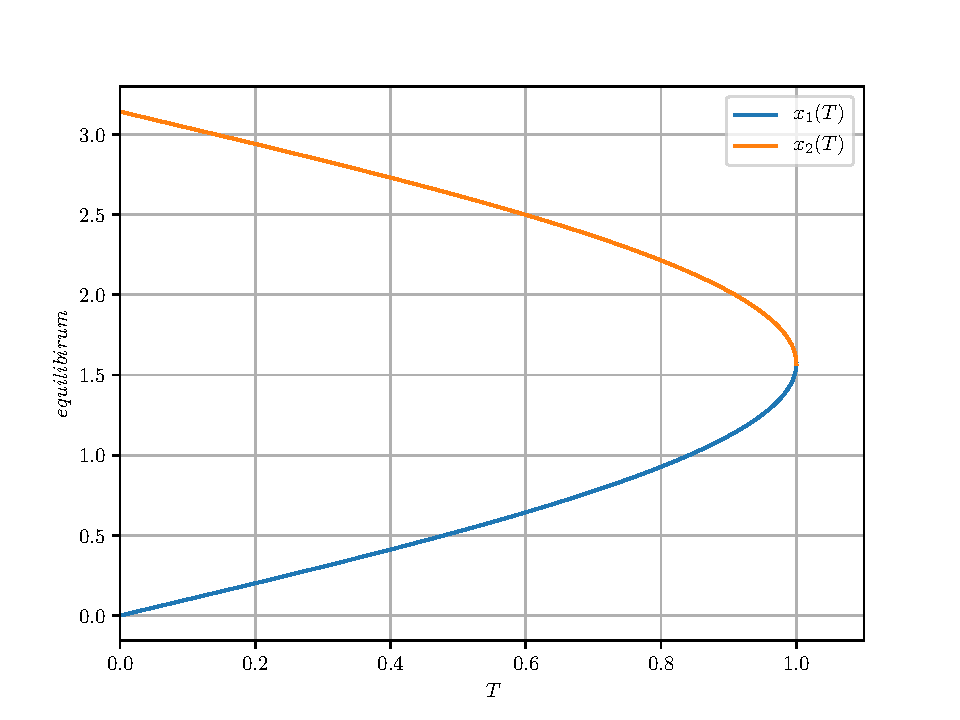
\includegraphics[width=0.9\textwidth]{figures/ex4_equilibriumPerTorque.pdf}
        \caption{\gr{Σημεία ισορροπίας συναρτήσει της ροπής \( T \) }}
        \label{fig:ex4_equilibriumPerTorque}
    \end{figure}
    Επικεντρώνουμε την προσοχή μας στο διάστημα \( (-\pi, \pi) \), δηλαδή για
    \( k = 0 \). Στο σχήμα~\ref{fig:ex4_equilibriumPerTorque} βλέπουμε την
    επιρροή που έχει η ροπή στα σημεία ισορροπίας. Καθώς αυξάνεται η ροπή τα
    δύο σημεία ισορροπίας \( x_1 \) και \( x_2 \) που αρχικά, για μηδενική
    ροπή ήταν στο \( (0, 0) \) και \( (\pi, 0) \) αντίστοιχα, πλησιάζουν μεταξύ τους
    μέχρι την οριακή τιμή της ροπής \( T = 1 \) όπου αυτά τα δύο σημεία
    ισορροπίας ταυτίζονται. Φυσικά όσο μεγαλώνει η ροπή, τόσο πλησιάζουν τα
    σημεία μεταξύ τους, που σημαίνει ότι όλο και πιο μικρές διαταραχές θα μας
    κάνουν το σύστημα ασταθές.
    \begin{figure}[h]
        \centering
        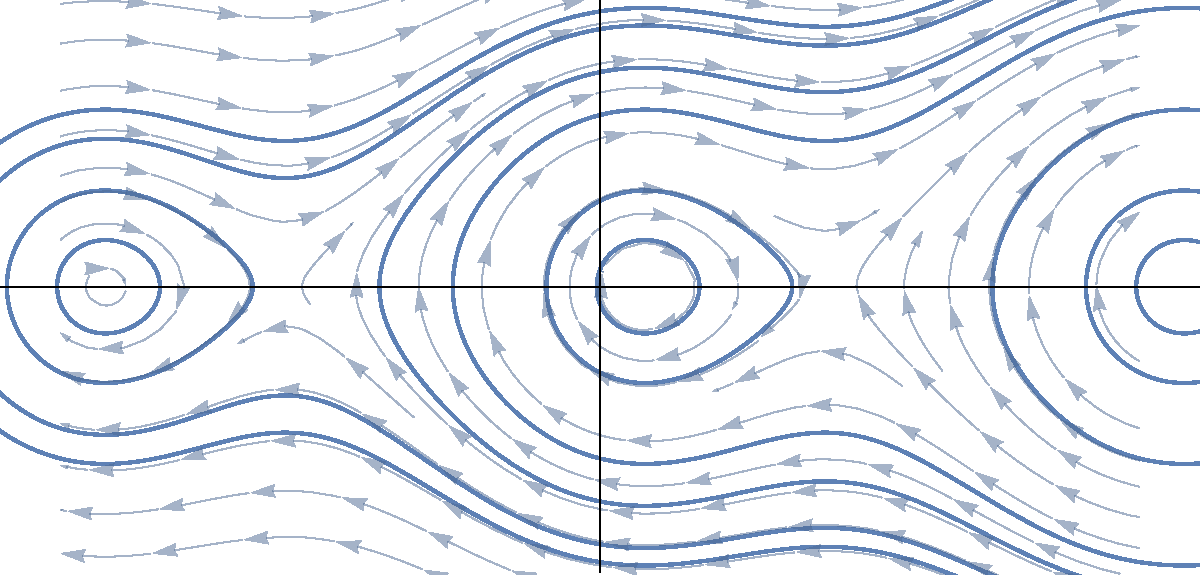
\includegraphics[width=0.8\textwidth]{figures/ex4_torque05Comb.pdf}
        \caption{\gr{Πορτρέτο κίνησης εκκρεμούς, \( a = 0, T = 0.5 \)}}
        \label{fig:ex4_torque05Comb}
    \end{figure}
    \begin{figure}[h]
        \centering
        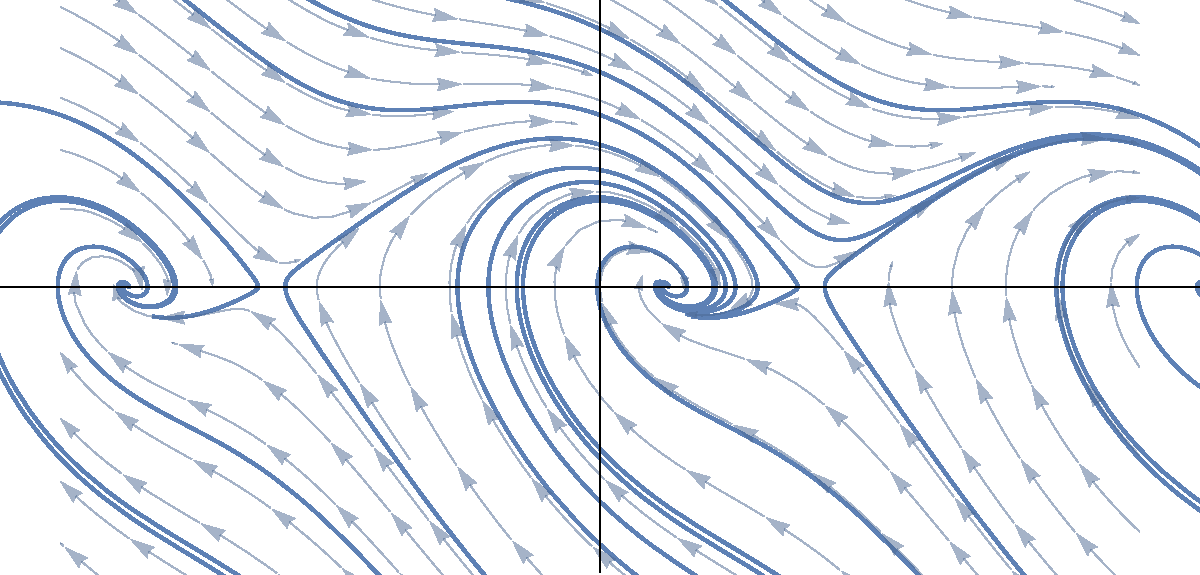
\includegraphics[width=0.8\textwidth]{figures/ex4_torque07damped07Comb.pdf}
        \caption{\gr{Πορτρέτο κίνησης εκκρεμούς, \( a = 0.7, T = 0.7 \)}}
        \label{fig:ex4_torque07damped07Comb}
    \end{figure}

    Στο σχήμα~\ref{fig:ex4_torque05Comb} βλέπουμε το πορτρέτο κίνησης για το
    εκκρεμές χωρίς απόσβεση και με ροπή \( T = 0.5 \). Παρατηρούμε ότι η ροπή
    μετακίνησε το σημείο ισορροπίας από το \( (0, 0) \) και το πήγε στο
    \( (0.52359, 0) \), ενώ το άλλο από το \( (\pi, 0) \) και το πήγε στο
    \( (2.6179, 0) \).

    Στο σχήμα~\ref{fig:ex4_torque05Comb} βλέπουμε το πορτρέτο κίνησης για το
    εκκρεμές με απόσβεση \( a = 0.7 \) και με ροπή \( T = 0.7 \). Παρατηρούμε
    ότι η ροπή μετακίνησε τα σημεία ισορροπίας ακόμα παραπάνω,
    από το \( (0, 0) \) στο \( (0.7753, 0) \), ενώ το άλλο από το \( (\pi, 0) \)
    στο \( (2.3661, 0) \). Όπως είναι φανερό από τα σχήματα, αλλά και από τις
    εξισώσεις, η ροπή δεν επηρεάζει τον τύπο των σημείων ισορροπίας.

    (β) \tl{ii}. Περνάμε στην περίπτωση όπου εφαρμόζεται μία σταθερή ροπή
    \( T > 1\) στο σύστημα, ώστε οι εξισώσεις να είναι
    \begin{align*}
        \dot{x} &= y \\
        \dot{y} &= -a y - \sin{x} + T.
    \end{align*}
    Υπολογίζοντας τα σημεία ισορροπίας προκύπτει
    \begin{align*}
        0 &= y \\
        0 &= -a y - \sin{x} + T,
    \end{align*}
    που συνεπάγεται
    \[
        \sin{x} = T.
    \]
    Η παραπάνω προφανώς για \( T > 1 \) δεν έχει λύσεις, και άρα το σύστημα δεν
    έχει σημεία ισορροπίας στην περίπτωση αυτή.
    \begin{figure}[h!]
        \centering
        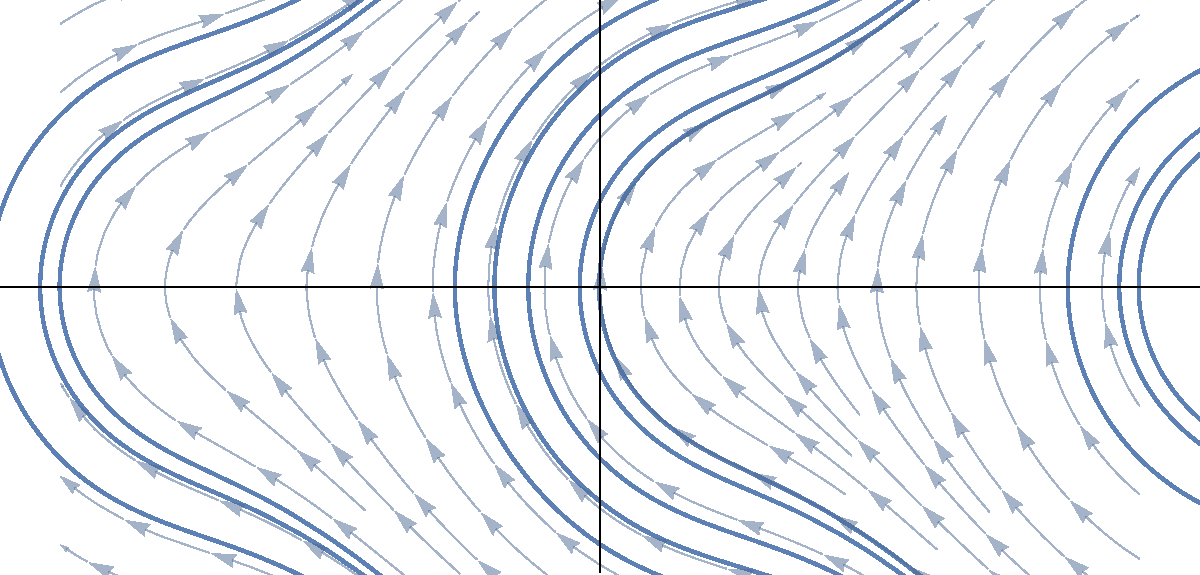
\includegraphics[width=0.8\textwidth]{figures/ex4_torque2Comb.pdf}
        \caption{\gr{Πορτρέτο κίνησης εκκρεμούς, \( a = 0, T = 2 \)}}
        \label{fig:ex4_torque2Comb}
    \end{figure}
    \begin{figure}[h!]
        \centering
        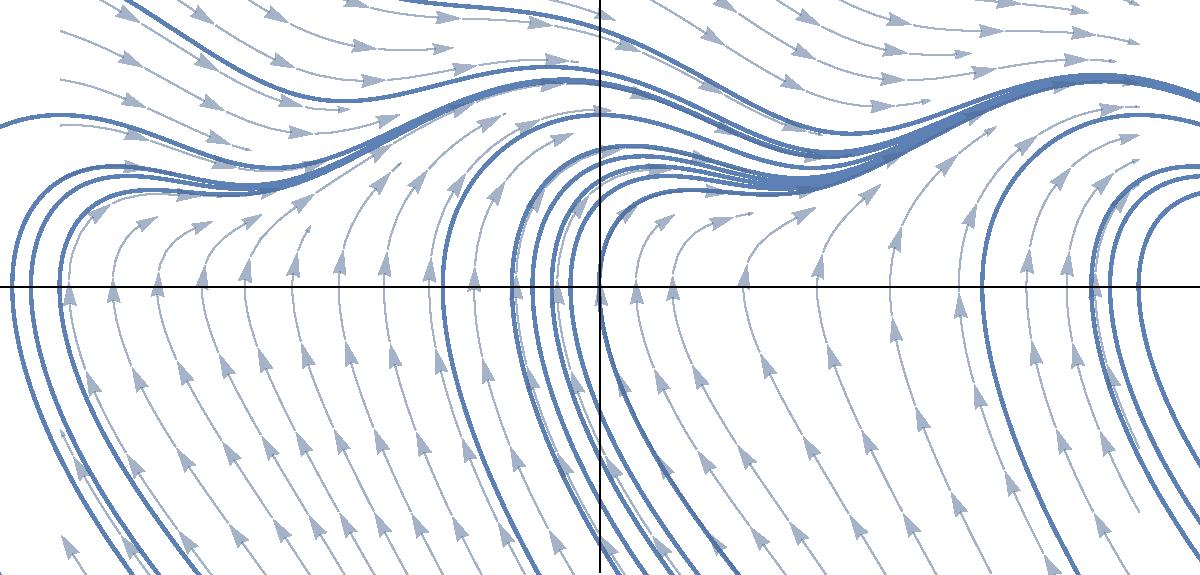
\includegraphics[width=0.8\textwidth]{figures/ex4_torque2damped1Comb.pdf}
        \caption{\gr{Πορτρέτο κίνησης εκκρεμούς, \( a = 1, T = 2 \)}}
        \label{fig:ex4_torque2damped1Comb}
    \end{figure}
    \begin{figure}[h!]
        \centering
        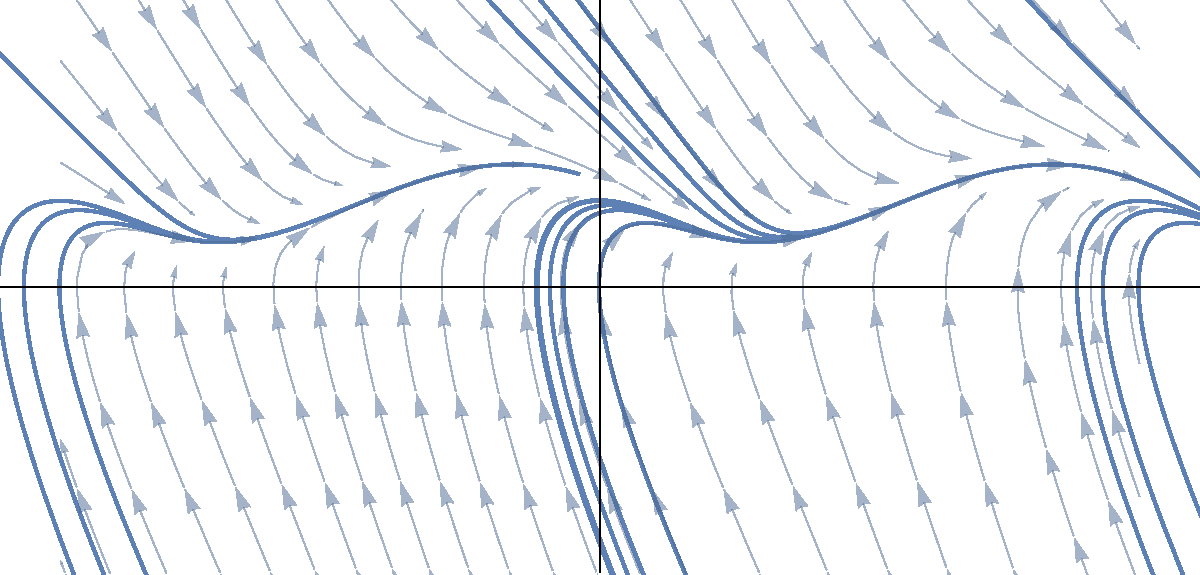
\includegraphics[width=0.8\textwidth]{figures/ex4_torque2damped2Comb.pdf}
        \caption{\gr{Πορτρέτο κίνησης εκκρεμούς, \( a = 2, T = 2 \)}}
        \label{fig:ex4_torque2damped2Comb}
    \end{figure}

    Στο σχήμα~\ref{fig:ex4_torque2Comb} βλέπουμε το πορτρέτο κίνησης για το
    εκκρεμές χωρίς απόσβεση και με ροπή \( T = 2 \). Παρατηρούμε ότι χωρίς
    απόσβεση το σύστημα είναι ασταθές.

    Στα σχήματα~\ref{fig:ex4_torque2damped1Comb}
    και~\ref{fig:ex4_torque2damped2Comb} βλέπουμε τα πορτρέτα κίνησης για το
    εκκρεμές με απόσβεση \( a = 1 \) και \( a = 2 \) αντίστοιχα και με ροπή
    \( T = 2 \). Παρατηρούμε ότι με την ύπαρξη της απόσβεσης και με την αύξηση
    αυτής, δημιουργείται ευσταθής οριακός κύκλος.
\end{solution}
